\chapter{High Low Guessing Game With Hints}
\label{chapter:hlggwh}
\graphicspath{ {./Lab05HighLowWithHints/Fig} }

\section{Outcomes and Objectives}

The outcome of this lab is to modify the high Low Guess
circuit to add increased functionality.
Through this process you will achieve the following
learning objectives.
\begin{itemize}
    \item \Paste{bok:CC_WireLogic}
    \item \Paste{bok:CC_Glue_Combo}
    \item \Paste{bok:CC_Combos}
    \item \Paste{VER:Test}
    \item\Paste{HDL:Pin}
\end{itemize}

\section{The Guessing Game with Hints}

This week's assignment asks you to add some enhanced functionality to
the guessing game. Since we are adding functionality, it's worth reviewing the
guessing game because we will use some of
the terms in the description of our enhanced functionality. The guessing game
starts with the secret keeper generating a \emph{secret number} between
{[}0 and 15{]}, inclusive. Once the \emph{secret number} is decided, the
guesser makes a \emph{guess}, a number in the interval {[}0 to 15{]}
inclusive, and tells this to the secret keeper. The secret keep then
replies to the guesser if \emph{guess} is less than, equal to, or
greater than the \emph{secret number}. The game continues with repeated
guesser/secret keeper exchange until the guesser correctly identifies
the \emph{secret number}.

In this lab assignment, you will add circuitry to provide an
indication of how far the user's guess is from the secret number by
telling them if their \emph{guess} is hot (close to the \emph{secret
number}), warm (kind-of close to the \emph{secret number}), or cold (far
away from the \emph{secret number}).

The user input and output, shown in Figure~\ref{fig:iOonDevBorad} are the same as last week's
assignment with the exception of the \textbf{hotCold} button and
\textbf{clue} 7-segment display.

\begin{figure}[ht]
    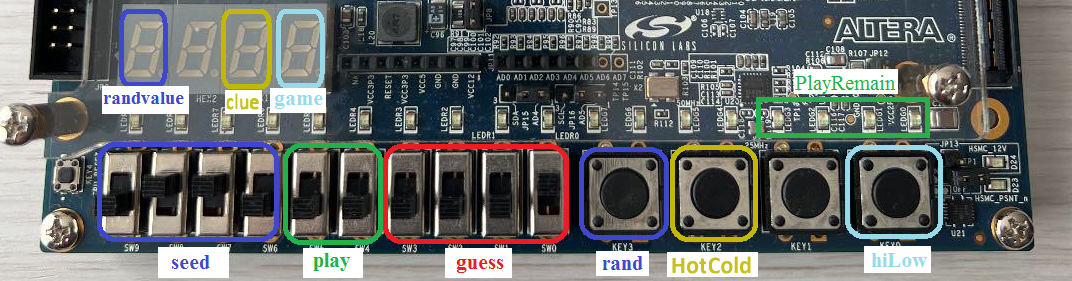
\includegraphics[width=0.8\paperwidth]{ image1.png}
    \caption{The input and output you should use to realize your digital system.}
    \label{fig:iOonDevBorad}
\end{figure}

The inputs and outputs include all the signals from last week's assignment
with the addition of a \textbf{hotCold} button and \textbf{clue} 7-segment
display.

The player can request a more refined evaluation of their guess by
pressing the \textbf{hotCold} button. To make this evaluation, the
absolute value of the difference between the \emph{guess} and
\emph{secret number} is computed.  This difference, called
\emph{difference} is compared against warmThreshold
and coldThreshold as shown in Figure~\ref{fig:guessThreshold}.
This figure an be interpreted as follows:

\begin{itemize}
    \item
        If difference $<$ warmThreshold the guess is Hot
    \item
        If (difference $\geq$ warmThreshold) and (difference $<$ coldThreshold) the guess is Warm
    \item
        If difference $\geq$ coldThreshold the guess is Cold
\end{itemize}

\begin{figure}[ht]
    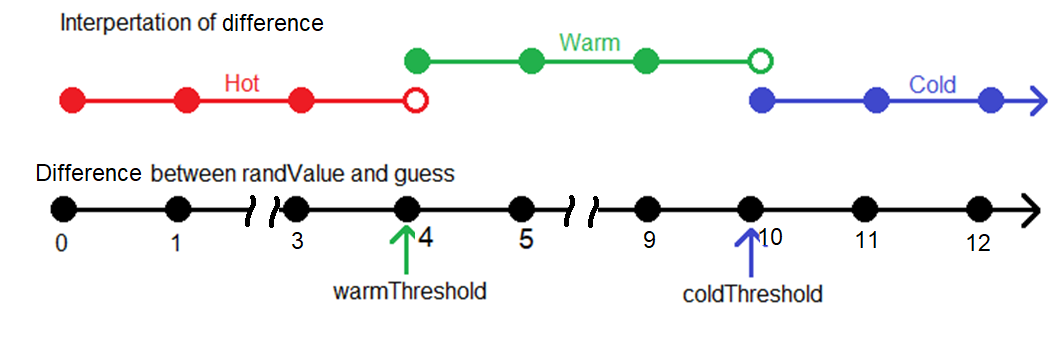
\includegraphics{ image2.png}
    \caption{The interpretation of the quality of a guess in terms of thresholds.}
    \label{fig:guessThreshold}
\end{figure}

Explore the relationship
between guess, secret number and the quality of the guess by completing
Table~\ref{table:applyGuessIntervals}. Assume a 4-bit word size for guess
and the secret number and use warmThreshold = 4 and ColdThreshold=10.

\begin{longtable}[]{@{}
        |  >{\raggedright\arraybackslash}p{(\columnwidth - 6\tabcolsep) * \real{0.2499}}|
        >{\raggedright\arraybackslash}p{(\columnwidth - 6\tabcolsep) * \real{0.2499}}|
        >{\raggedright\arraybackslash}p{(\columnwidth - 6\tabcolsep) * \real{0.2501}}|
    >{\raggedright\arraybackslash}p{(\columnwidth - 6\tabcolsep) * \real{0.2501}}|@{}}
    \caption{Determine the quality of a guess at the secret number. Your answer may be
    a number, pair of numbers, a range or a pair of ranges}
    \label{table:applyGuessIntervals}
    \tabularnewline
    \toprule()
    \begin{minipage}[b]{\linewidth}\raggedright
        \emph{guess}
    \end{minipage} &
    \begin{minipage}[b]{\linewidth}\raggedright
        \emph{secret number}
    \end{minipage} &
    \begin{minipage}[b]{\linewidth}\raggedright
        difference
    \end{minipage} &
    \begin{minipage}[b]{\linewidth}\raggedright
        Quality
    \end{minipage} \\
    \midrule()
    \endfirsthead
    \toprule()
    \begin{minipage}[b]{\linewidth}\raggedright
        \emph{guess}
    \end{minipage} &
    \begin{minipage}[b]{\linewidth}\raggedright
        \emph{secret number}
    \end{minipage} &
    \begin{minipage}[b]{\linewidth}\raggedright
        difference
    \end{minipage} &
    \begin{minipage}[b]{\linewidth}\raggedright
        Quality
    \end{minipage} \\
    \midrule()
    \endhead
    14 & 11 & & \\ \hline
    8 & 12 & & \\ \hline
    4 & 14 & & \\ \hline
    8 & & 2 & Hot \\ \hline
    & 8 & {[}4 to 9{]} & Warm \\ \hline
    & 2 & {[}10 to 15{]} & Cold \\
    \bottomrule()
\end{longtable}

The 7-segment display called clue will communicate the quality of the
user's guess to the user. It will do this by displaying `C' if the guess
is \textbf{\uline{C}}old, `A' if the guess is w\textbf{\uline{A}}rm, `H'
if the guess is \textbf{\uline{H}}ot.

\section{System Architecture}
You will use the system
architecture shown in Figure~\ref{fig:guessWithHintSystemArch} to
design your circuit.

\begin{figure}[ht]
    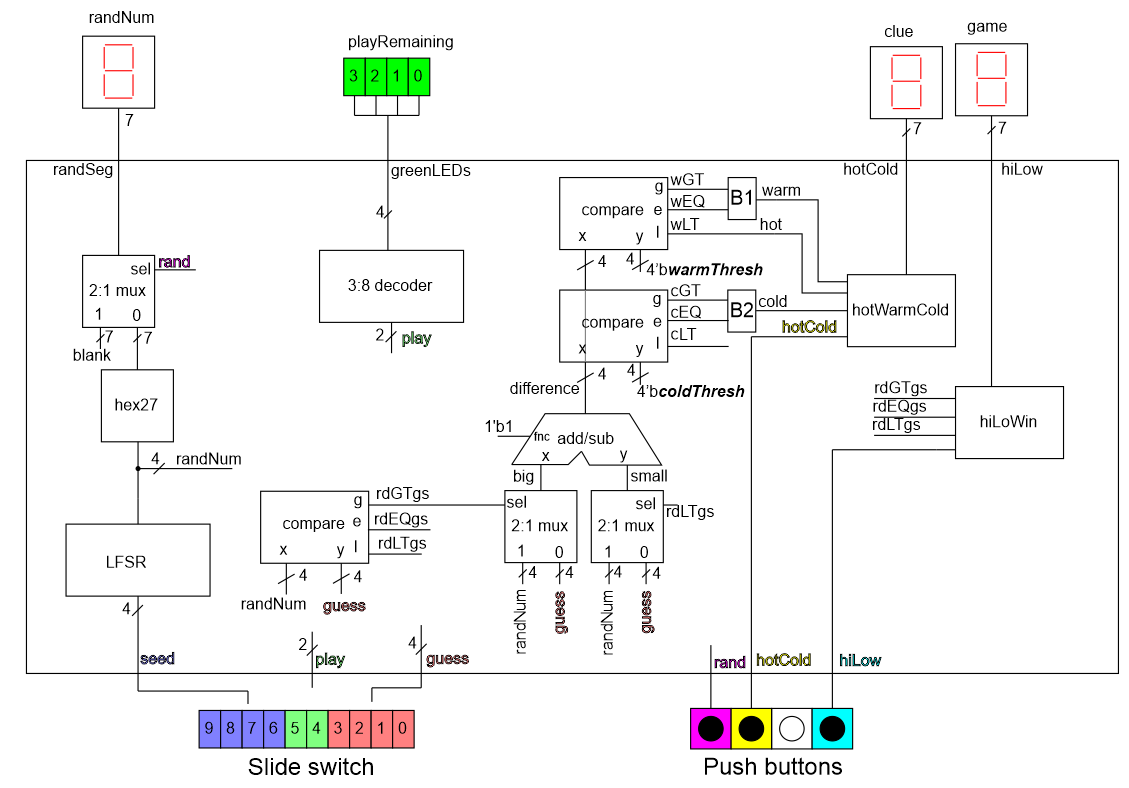
\includegraphics[width=6.50278in,height=4.42708in]{ image3.png}
    \caption{System architecture for the guessing game with hint. }
    \label{fig:guessWithHintSystemArch}
\end{figure}

You should use last week's lab as a starting point. The new circuitry is shown in the middle of
Figure~\ref{fig:guessWithHintSystemArch}.  Let's walk through the new circuitry
to understand what it does to provide a hint about the quality of the user's guess.

Let's start by examining the output of the add/sub, \emph{difference} which is the absolute
value of the difference between the \emph{randNum} and \emph{guess}.  It is computed
by taking the difference between the larger of \emph{randNum} and \emph{guess} and
subtracting the smaller of \emph{randNum} and \emph{guess}.  The add/sub is hardwired
to subtract because it's fun input is hardwired to 1'b1, hence it is always computing the
diferene between its \emph{x,y} inputs, \emph{big-small}.

The 2:1 mux in front of the add/sub's \emph{x} input passes \emph{randNum} to its
output, called \emph{big}, when the comparator to its left outputs 1.  This comparator
outputs 1 when \emph{randNum} is greater than \emph{guess}.  Hence when \emph{randNum}
is larger it is the \emph{big} output.

The output of the 2:1 mux in front of the add/sub's \emph{y} input, \emph{small} follows
a similar logical organization, but uses the less than output of the comparator to select the
smaller of \emph{randNum} or \emph{guess} to pass to the \emph{small} output.

Now that we have \emph{difference} computed correctly, let's see how it's used
to inform the user of the quality of their guess. The
\emph{difference} is compared to the warmThreshold and coldThreshold
using a pair of comparators. Through some logic that you will design you
will create three signals \emph{hot, warm, cold} which are based on the
relationship you examined in Figure~\ref{fig:guessThreshold}.

\section{Module: 2:1 Mux}
This module was discussed in Lab 4.

\section{Module: Compare}
This module was discussed in Lab 4.

\section{Module: Add/Sub }

A N-bit adder subtractor is a basic building block in many digital
systems. The N-bit adder subtractor shown adds its N-bit
input x and y when fnc = 0 and subtracts y from x when func=1. When
the inputs and output are interpreted as a 2's complement values, the
sovf output equals 1 when the computation results in an overflow. When
the inputs and output are interpreted as binary numbers, the uovf output
equals 1 when the computation results in an overflow.

The Verilog code for the N-bit adder subtractor is on Canvas. Since the
adder subtractor uses full-adders in its construction, you will need to
include the full adder module contained in the file fullAdder.v in your
project. Listing 2 shows the module declaration for the genericAdderSubtractor.
The module
instantiation shown in Listing 2 corresponds to the system architecture
shown in Figure~\ref{fig:guessWithHintSystemArch}. Since the inputs to the adder subtractor in the
system architecture will not generate overflow, the overflow outputs
from this adder subtractor are not needed. When you do not need an
output from a module, you can leave its parameter slot unfilled. This
explains the pair of empty fields at the end of the module instantiation
shown in Listing~\ref{listing:adderSubtractor}.

\begin{lstlisting}[language=Verilog,
 caption={Top, module definition for an adder subtractor.  Bottom, module instantation
 of the adder subtractor in Figure~\ref{fig:guessWithHintSystemArch}.},
 label={listing:adderSubtractor},
 frame=single]
// Module definition for the adder subtractor
module genericAdderSubtractor(a, b, fnc, sumDiff, sovf, uovf);

// Module instantiation for an adder subtractor in hiLow digital circuit
genericAdderSubtractor #(4) prox(big, small, 1'b1, difference, , );
\end{lstlisting}

Like the mux and comparator, the adder subtractor is a generic module.
This means that you need to specify the vector width of the \textbf{X}
and \textbf{Y} inputs and \textbf{sumDiff} output using the \#()
specifier. Pay close attention to match the value of this generic and
the size of the input and output vectors.

\section{Logic: hotWarmCold}

The goal of this section is to determine the logic inside the hotWarmCold logic block
in Figure~\ref{fig:guessWithHintSystemArch}.  To do this you will first need to form three
signals, \emph{hot}, \emph{warm}, and \emph{cold}.  These three signals describe how close the
\emph{guess} is from \emph{randNum}. We will call the comparator that compares \emph{difference}
and \emph{warmThresh}, the warm comparator and call its three outputs wGT, wEQ and wLT.
The other comparator is the cold comparator and its outputs prefixed with  lowercase ``c''.

The values of \emph{warmThresh and coldThresh} are set using the signal declaration
and signal assignment statements shown in Listing~\ref{listing:guessThresholds}.

\begin{lstlisting}[language=Verilog,
 caption={The signal declaration and assignment for guess thresholds.},
 label={listing:guessThresholds},
 frame=single]
    wire [3:0] warmThreshold, coldThreshold;
    assign warmThreshold = 4'b0100;
    assign coldThreshold = 4'b1010;
\end{lstlisting}

The warm and cold comparators generate a total of 6 signals, some of which are
sent to the logic block B1 and B2 to form the warm and cold signals - the logic for the
hot signal is given to you in Figure~\ref{fig:guessWithHintSystemArch}.

To understand the logic inside the B1 and B2 logic blocks let's work through a
set of examples in Table~\ref{table:fillInCompareOperations}.  In these examples
you will let:
\begin{itemize}
    \item \emph{coldThresh} = 10
    \item \emph{warmThresh} = 4
    \item \emph{difference} = 9
\end{itemize}

as a first step, let's determine the outputs of the warm comprarator.
The x input o the waarm omprator is equal to 9 (the value of \emph{difference})
and the y input equals 4 (the value of \emph{warmThresh}). Since 9 is
greater than 4, then:
\begin{itemize}
    \item wGT = 1
    \item wEQ =0
    \item wLT =0
\end{itemize}

Using similr reasoning we ind that:
\begin{itemize}
    \item cGT = 0
    \item cEQ =0
    \item cLT =1
\end{itemize}

Finally, since \emph{difference} equals 9 and this is between the warm
and cold thresholds, the quality of the guess is warm, so we set this output
equal to 1 and hot and cold to 0.

\begin{longtable}[]{@{}
        | >{\raggedright\arraybackslash}p{(\columnwidth - 18\tabcolsep) * \real{0.1110}}|
        >{\raggedright\arraybackslash}p{(\columnwidth - 18\tabcolsep) * \real{0.1004}}|
        >{\raggedright\arraybackslash}p{(\columnwidth - 18\tabcolsep) * \real{0.1004}}|
        >{\raggedright\arraybackslash}p{(\columnwidth - 18\tabcolsep) * \real{0.1005}}|
        >{\raggedright\arraybackslash}p{(\columnwidth - 18\tabcolsep) * \real{0.1004}}|
        >{\raggedright\arraybackslash}p{(\columnwidth - 18\tabcolsep) * \real{0.1004}}|
        >{\raggedright\arraybackslash}p{(\columnwidth - 18\tabcolsep) * \real{0.1005}}|
        >{\raggedright\arraybackslash}p{(\columnwidth - 18\tabcolsep) * \real{0.0957}}|
        >{\raggedright\arraybackslash}p{(\columnwidth - 18\tabcolsep) * \real{0.0957}}|
    >{\raggedright\arraybackslash}p{(\columnwidth - 18\tabcolsep) * \real{0.0951}}@{}|}
    \caption{Complete the following table, let warmThresh = 4 and coldThresh = 10.  Leave
    comprator outputs which re 0 blank.}\label{table:fillInCompareOperations}\tabularnewline
    \toprule()
    \multirow{2}{*}{difference} &
    \multicolumn{3}{|c|}{warmThresh comparator} &
    \multicolumn{3}{|c|}{coldThresh comparator} &
    \multirow{2}{*}{Hot} &
    \multirow{2}{*}{Warm} &
    \multirow{2}{*}{Cold} \\ \cline{2-7}
    & wGT & wEQ & wLT & cGT & cEQ &  \\ \cline{2-7}
    \midrule()
    \endfirsthead
    \toprule()
    \multirow{2}{*}{difference} &
    \multicolumn{3}{|c|}{warmThresh comparator} &
    \multicolumn{3}{|c|}{coldThresh comparator} &
    \multirow{2}{*}{Hot} &
    \multirow{2}{*}{Warm} &
    \multirow{2}{*}{Cold} \\ \cline{2-7}
    & wGT & wEQ & wLT & cGT & cEQ & cLT \\ \cline{2-7}
    \midrule()
    \endhead
    3 & & & & & & & & & \\ \hline
    4 & & & & & & & & & \\ \hline
    5 & & & & & & & & & \\ \hline
    9 & 1 & & & & & 1 & & 1 & \\ \hline
    10 & & & & & & & & & \\ \hline
    11 & & & & & & & & & \\
    \bottomrule()
\end{longtable}

Now, you need to use the values in Table~\ref{table:fillInCompareOperations} to determine the logic for
each of the three outputs from the ``discrete logic'' block shown in
Figure~\ref{fig:guessWithHintSystemArch}. To do this write an expression using AND and OR to
describe when that
output equals 1.

\protect\hypertarget{hotWarmCold_Logic}{}{}
\begin{verbatim}
    cold =                               // write logic description
    warm =                            // write logic description
    hot = wLT;                       // given to you in  Figure~\ref{fig:guessWithHintSystemArch}
\end{verbatim}

For the hotWarmCold block of code:

\begin{itemize}
    \item
        Make three assign statements, one for hot, warm and cold
    \item
        Use only \& and \textbar{} operations.
    \item
        Use parenthesis to ensure proper order of operation.
    \item
        The \emph{hot}, \emph{warm} and \emph{cold} signals should be ``wire''
        type.
\end{itemize}

One you hve the logi or the hot/wrm nd cold signals you an strt building the
hotWrmold logi block.
You will implement the hotWarmCold logic using an always/case statement
that uses the 3-bit vector \emph{hot}, \emph{warm} and \emph{cold} to form
the 7-segment output shown in Figure~\ref{figure:hiLoHintSevenSeg} when
the \emph{hotCold} button is pressed. The 7-segment display should be blank
when the \emph{hotCold} button is unpressed.

\begin{figure}[ht]
    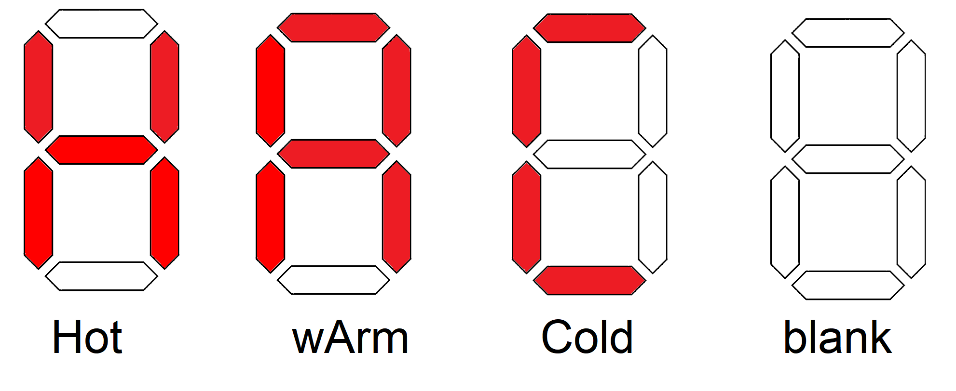
\includegraphics[width=0.5\paperwidth]{ image5.png}
    \caption{The illuminated patterns to inform the guesser about the magnitude of their guess.}
    \label{figure:hiLoHintSevenSeg}
\end{figure}

For this block of code:

\begin{itemize}
    \item
        Use an always/case statement.
    \item
        Form a 4-bit vector from the \emph{hot}, \emph{warm}, \emph{cold}
        signals and the \textbf{hotCold} button.
    \item
        Use this 4-bit vector as the input to the always/case statement.
    \item
        Make sure that the output signal has ``reg'' type.
    \item
        Include inline comments prior to the always/case statement describing
        the pattern that is displayed on the 7-segment display for each
        possible output. An example is given in Listing~\ref{listing:hotColdGuess}.
\end{itemize}

\begin{lstlisting}[language=Verilog,
 caption={A comment block describing the pattern of illuminated segment for each guess hint..},
 label={listing:hotColdGuess},
 frame=single]
//*********************************************
// Logic to display the quality of the guess
//    Hot  = `H' = <show binary code>
//    wArm = `A' = <show binary code>
//    Cold = `C' = <show binary code>
//
//         hex[0]
//         -----
//    hex[5]    |    |    hex[1]
//        |    |
//         -----    hex[6]
//    hex[4]    |    |
//        |    |    hex[2]
//         -----
//         hex[3]
//*********************************************
\end{lstlisting}

\section{Module: hiLow}
This is the top-level module in Figure~\ref{fig:guessWithHintSystemArch}, the outermost
block. \uline{If you were not able to get the previous lab working}, just
implement the functionality identified in this assignment and make the
\emph{randNum} come directly from the seed switch. In this case, you
should use the top module declaration in Listing~\ref{listing:hiLowModule}. If you got the
previous lab working correctly, then you should use the bottom
declaration in Listing~\ref{listing:hiLowModule}.

\begin{lstlisting}[language=Verilog,
 caption={The module declaration for the enhanced hiLow module if you did or did
 not get the previous lab working.},
 label={listing:hiLowModule},
basicstyle=\tiny\ttfamily,
 frame=single]

 // if you did not get the previous lab working, then use this module declaration
module hiLow(seedSwitch, guessSwitch, hotColdBut, hotColdSeg);

// If you successfully completed previous lab, then use this module declaration (with no line break)
module hiLow(seedSwitch, playSwitch, guessSwitch, randBut, hotColdBut, hiLowBut, randMsbSeg, randLsbSeg,
                    greenLEDs, hotColdSeg, hiLowSeg);
 \end{lstlisting}

For this block of code:

\begin{itemize}
    \item
        Instantiate genericMux2x1 using the module provided in the previous
        lab.
    \item
        Instantiate genericCompare using the module provided in the previous
        lab.
    \item
        Instantiate genericAddSub using the module provided in the Canvas
        folder for this lab.
    \item
        Make sure to include the fullAdder module in your project.
    \item
        Use descriptive names for internal signal.
    \item
        Use descriptive names for component instance names.
\end{itemize}

\section{Testbench}

The testbench checks hot, warm and cold for guesses that
are too high and too low. I carefully selected these values to check the
edge cases, meaning on either side of the warm and cold thresholds.
\begin{verbatim}
    warmThresh = 4'b0110 = 4
    coldThresh = 4'b0110 = 10
\end{verbatim}

Table~\ref{table:hiLowTestbenchValues} contains the values that you will use to test your circuit.
Before using the testbench, you need to understand what your circuit
should output. The signal names in the top row of Table~\ref{table:hiLowTestbenchValues} are borrowed
from the system architecture in Figure~\ref{fig:guessWithHintSystemArch}. Fill in the missing binary and
decimal values for the cells in the guess, big, small and difference
columns. In the Comment column, put the quality of the guess as either
``Hot'', ``Warm'' or ``Cold''.

\begin{longtable}[]{@{}
        | >{\raggedright\arraybackslash}p{(\columnwidth - 14\tabcolsep) * \real{0.0742}}|
        >{\raggedright\arraybackslash}p{(\columnwidth - 14\tabcolsep) * \real{0.1258}}|
        >{\raggedright\arraybackslash}p{(\columnwidth - 14\tabcolsep) * \real{0.1258}}|
        >{\raggedright\arraybackslash}p{(\columnwidth - 14\tabcolsep) * \real{0.1392}}|
        >{\raggedright\arraybackslash}p{(\columnwidth - 14\tabcolsep) * \real{0.1392}}|
        >{\raggedright\arraybackslash}p{(\columnwidth - 14\tabcolsep) * \real{0.1392}}|
        >{\raggedright\arraybackslash}p{(\columnwidth - 14\tabcolsep) * \real{0.1392}}|
    >{\raggedright\arraybackslash}p{(\columnwidth - 14\tabcolsep) * \real{0.1174}}@{}|}
    \caption{Table : The values used in the hiLow testbench.}\label{table:hiLowTestbenchValues}\tabularnewline
    \toprule()
    Test & seed & randNum & guess & big & small & Difference & Comment \\
    \midrule()
    \endfirsthead
    \toprule()
    Test & seed & randNum & guess & big & small & Difference & Comment \\
    \midrule()
    \endhead
    1  &
    \multirow{5}{*}{4'b1010} &
    \multirow{5}{*}{4'b0100 } &
    4'b1111 &  &
    \multirow{5}{*}{} & &                  \\ \cline{1-1}\cline{4-5}\cline{7-8}
    2 & & & =14         &  & &  &         \\ \cline{1-1}\cline{4-5}\cline{7-8}
    3 & & & 4'b1101 =     &  & &  &          \\ \cline{1-1}\cline{4-5}\cline{7-8}
    4 & & & 4'b1000 =    & & &  &          \\ \cline{1-1}\cline{4-5}\cline{7-8}
    5 & & & 4'b0111 =     &  & &  &          \\ \hline

    6 &
    \multirow{6}{*}{4'b1111} &
    \multirow{6}{*}{4'b1110} &
    4'b0011 &
    \multirow{6}{*}{} &  &  &  \\ \cline{1-1}\cline{4-4}\cline{6-8}

    7  & & &  =4 & &  &  & \\ \cline{1-1}\cline{4-4}\cline{6-8}
    8  & & & =5 & & &  & \\ \cline{1-1}\cline{4-4}\cline{6-8}
    9  & & & 4'b1010 = & &  & &  \\ \cline{1-1}\cline{4-4}\cline{6-8}
    10 & & & 4'b1011 = & & & & \\ \cline{1-1}\cline{4-4}\cline{6-8}
    11 & & & 4'b1110 = & & & & \\
    \bottomrule()
\end{longtable}

When you figure out what the testbench will output, its time to run it.
Use the testbench provided on Canvas. Produce a timing diagram with the
following waves with the correct radix and color and order the
traces from top to bottom as

\begin{tabular}{p{4cm}p{4cm}p{4cm}}
    signal & radix & trace color \\ \hline
    seedSwitch  &  unsigned & Green  \\
    randNum  &  unsigned  & Lime green  \\
    GuessSwitch  &  unsigned  & Lime green  \\
    Big   & unsigned &  Cyan  \\
    Small  &  unsigned &  Cyan  \\
    Difference  &  unsigned &  Blue  \\
    hotWire  & default &  Orange  \\
    warmWire  & default &  Orange  \\
    coldWire  & default &  Orange  \\
    hotColdSeg  & hexadecimal &  Red  \\
\end{tabular}

When compete, your testbench should look like the timing diagram in
Figure~\ref{fig:guessTiming}.

\begin{figure}[ht]
    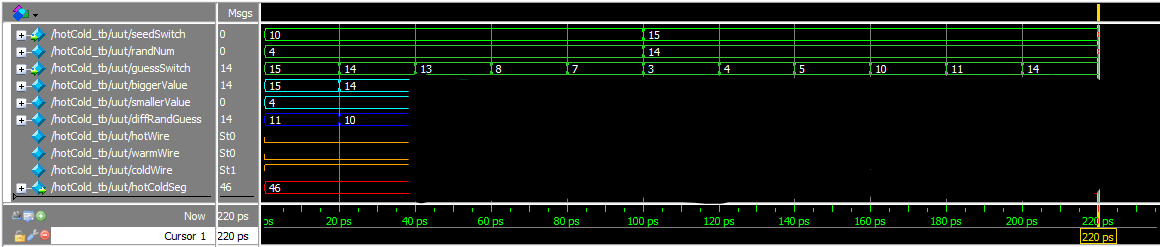
\includegraphics{ image7.png}
    \caption{A partially obscured timing diagram generated by the testbench.}
    \label{fig:guessTiming}
\end{figure}

\section{Pin-Assignment and Synthesis}

Use the image of the C5G Development Board in Figure~\ref{fig:iOonDevBorad} and the information
in the User Guide to determine the FPGA pins associated with the input
and output devices used by the hiLow module.

\begin{longtable}[]{@{}
        |  >{\raggedright\arraybackslash}p{(\columnwidth - 6\tabcolsep) * \real{0.2571}}|
        >{\raggedright\arraybackslash}p{(\columnwidth - 6\tabcolsep) * \real{0.2814}}|
        >{\raggedright\arraybackslash}p{(\columnwidth - 6\tabcolsep) * \real{0.2430}}|
    >{\raggedright\arraybackslash}p{(\columnwidth - 6\tabcolsep) * \real{0.2185}}|@{}}
    \caption{Pin-assignment for the High Low Guessing Game with Hints.}\label{table:hiLowPinAssignment}\tabularnewline
    \toprule()
    \begin{minipage}[b]{\linewidth}\raggedright
        Segment
    \end{minipage} &
    \begin{minipage}[b]{\linewidth}\raggedright
        randSeg
    \end{minipage} &
    \begin{minipage}[b]{\linewidth}\raggedright
        hotColdSeg
    \end{minipage} &
    \begin{minipage}[b]{\linewidth}\raggedright
        hiLowSeg
    \end{minipage} \\
    \midrule()
    \endhead
    seg{[}6{]} & AC22 & &  \\ \hline
    seg{[}5{]} &     & &  \\ \hline
    seg{[}4{]} &  & &  \\ \hline
    seg{[}3{]} &  & & W18 \\ \hline
    seg{[}2{]} & AA23 & &  \\ \hline
    seg{[}1{]} &  & &  \\ \hline
    seg{[}0{]} &  & & V19 \\
    \bottomrule()
\end{longtable}

\begin{longtable}[]{@{}
        |  >{\raggedright\arraybackslash}p{(\columnwidth - 6\tabcolsep) * \real{0.2596}}|
        >{\raggedright\arraybackslash}p{(\columnwidth - 6\tabcolsep) * \real{0.2505}}|
        >{\raggedright\arraybackslash}p{(\columnwidth - 6\tabcolsep) * \real{0.2542}}|
    >{\raggedright\arraybackslash}p{(\columnwidth - 6\tabcolsep) * \real{0.2357}}|@{}}
    \toprule()
    \begin{minipage}[b]{\linewidth}\raggedright
    \end{minipage} &
    \begin{minipage}[b]{\linewidth}\raggedright
        seedSwitch
    \end{minipage} &
    \begin{minipage}[b]{\linewidth}\raggedright
        playSwitch
    \end{minipage} &
    \begin{minipage}[b]{\linewidth}\raggedright
        guessSwitch
    \end{minipage} \\
    \midrule()
    \endhead
    slide{[}3{]} & AE19 & N/A &  \\ \hline
    slide{[}2{]} &  & N/A &  \\ \hline
    slide{[}1{]} &  &  & AE10 \\ \hline
    slide{[}0{]} &  & W11 &  \\
    \bottomrule()
\end{longtable}

\begin{longtable}[]{@{}
        |  >{\raggedright\arraybackslash}p{(\columnwidth - 4\tabcolsep) * \real{0.3334}}|
        >{\raggedright\arraybackslash}p{(\columnwidth - 4\tabcolsep) * \real{0.3334}}|
    >{\raggedright\arraybackslash}p{(\columnwidth - 4\tabcolsep) * \real{0.3333}}|@{}}
    \toprule()
    \begin{minipage}[b]{\linewidth}\raggedright
        randBut
    \end{minipage} &
    \begin{minipage}[b]{\linewidth}\raggedright
        Key{[}3{]}
    \end{minipage} &
    \begin{minipage}[b]{\linewidth}\raggedright
        Y16
    \end{minipage} \\
    \midrule()
    \endhead
    \begin{minipage}[t]{\linewidth}\raggedright
        hotColdBut
    \end{minipage} & Key{[}2{]} & \\ \hline
    \begin{minipage}[t]{\linewidth}\raggedright
        hiLowBut
    \end{minipage} & Key{[}0{]} &  \\
    \bottomrule()
\end{longtable}

\begin{longtable}[]{@{}
        | >{\raggedright\arraybackslash}p{(\columnwidth - 6\tabcolsep) * \real{0.2499}}|
        >{\raggedright\arraybackslash}p{(\columnwidth - 6\tabcolsep) * \real{0.2499}}|
        >{\raggedright\arraybackslash}p{(\columnwidth - 6\tabcolsep) * \real{0.2501}}|
    >{\raggedright\arraybackslash}p{(\columnwidth - 6\tabcolsep) * \real{0.2501}}|@{}}
    \toprule()
    \begin{minipage}[b]{\linewidth}\raggedright
        G{[}3{]}
    \end{minipage} &
    \begin{minipage}[b]{\linewidth}\raggedright
        G{[}2{]}
    \end{minipage} &
    \begin{minipage}[b]{\linewidth}\raggedright
        G{[}1{]}
    \end{minipage} &
    \begin{minipage}[b]{\linewidth}\raggedright
        G{[}0{]}
    \end{minipage} \\
    \midrule()
    \endhead
    E9 &  &  &  \\
    \bottomrule()
\end{longtable}

Complete the pin-assignment in Quartus, compile your design and download to the
FGPA development boards.  If you are having difficulty getting your circuit to work
correctly, please refer to Section~\ref{section:hiLowHintDebugging} for some
useful debugging tips.

Once you get your design working, demonstrate it to a member of the
lab team.

\section{Turn in}

You may work in teams of at most two. Make a record of your response to
the items below and turn them in a single copy as your team's solution
on Canvas using the instructions posted there. Include the names of both
team members at the top of your solutions. Use complete English
sentences to introduce what each of the following listed items (below)
is and how it was derived. In addition to this submission, you will be
expected to demonstrate your circuit at the beginning of your lab
section next week.

\subsubsection{System Architecture}
\begin{itemize}
    \item Complete Table~\ref{table:applyGuessIntervals}.
\end{itemize}

\subsubsection{Discrete Logic block}
\begin{itemize}
    \item Complete Table~\ref{table:fillInCompareOperations}

    \item \protect\hyperlink{hotWarmCold_Logic}{Link} Logic for hot, warm, and cold signals
\end{itemize}

\subsubsection{Module: hiLow}

\begin{itemize}
    \item
        \protect\hyperlink{hilow-module}{Link} Verilog code for the body of
        the hiLow module (courier 8-point font single spaced), leave out
        header comments.
    \item  Complete Table~\ref{table:hiLowTestbenchValues}.
    \item  \protect\hyperlink{hilow_tb-module}{Link}  Complete testbench timing diagram.
\end{itemize}

\subsubsection{Pin-Assignment and Synthesis}
\begin{itemize}
    \item Complete pin-assignment table or ll the signals in Table~\ref{table:hiLowPinAssignment}.
    \item Demonstrate your completed circuit to a lab team member.
\end{itemize}

\section{Debugging Tips}
\label{section:hiLowHintDebugging}

Even when your program executes successfully, you may get the warnings shown in
Figure~\ref{fig:messageConsole}. These are mainly the result of the unused overflow outputs
from the adder subtractor. You can filter out all the compile messages
by clicking on the yellow triangle (with the blue three in this case) on
the top line of the console window. Note, if there are several related
warnings, they will have one top-level warning with all the instances
accessible by clicking the expander arrow (it looks like
``\textgreater'') to the left of the warning triangle.

\begin{figure}[ht]
    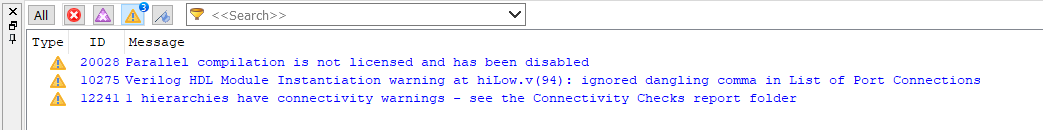
\includegraphics{image8.png}
    \caption{The messages console filtered by warnings.}
    \label{fig:messageConsole}
\end{figure}

The Connectivity Checks folder in the Compilation Report will help
you quickly track down errors. To use it, open the Connectivity
Checks folder, click on a Port Connectivity Checks item and read the
report in the right pane. In the report shown in Figure~\ref{fig:connectivityCheck}, I selected
the genericAdderSubtractor, note the fnc input is hardwired to 1 so that it
always subtracts. This report also shows that the overflow outputs are
unconnected because we left them open using a pair of commas talked
about earlier.

\begin{figure}[ht]
    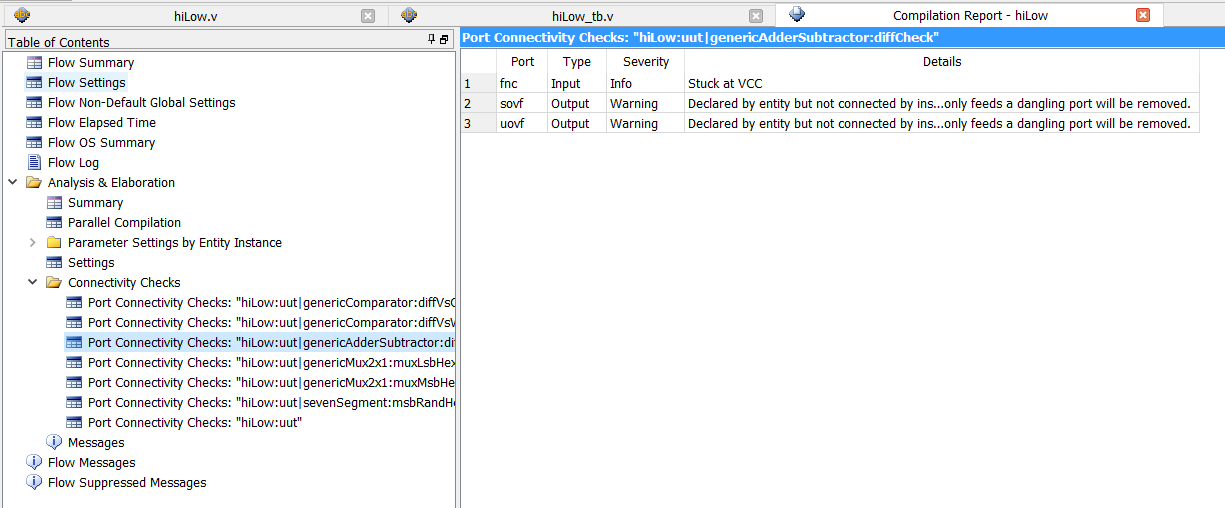
\includegraphics{ image9.png}
    \caption{Connectivity Checks report for a working hiLow circuit.}
    \label{fig:connectivityCheck}
\end{figure}
